\documentclass[conference]{IEEEtran}
\IEEEoverridecommandlockouts
\usepackage{cite}
\usepackage{amsmath,amssymb,amsfonts}
\usepackage{algorithmic}
\usepackage{graphicx}
\usepackage{textcomp}
\usepackage{xcolor}
\usepackage{tikz}
\usetikzlibrary{patterns,decorations.pathmorphing}
\def\BibTeX{{\rm B\kern-.05em{\sc i\kern-.025em b}\kern-.08em
    T\kern-.1667em\lower.7ex\hbox{E}\kern-.125emX}}
\begin{document}

\title{Overview of Inverse Finite Element Method for Beam Analysis}



\author{\IEEEauthorblockN{Antoine Grosse}
\IEEEauthorblockA{\textit{Institutt for marin teknikk (IMT)} \\
\textit{NTNU}\\
Trondheim, Norway \\
antoine.grosse@ntnu.no}
\and
\IEEEauthorblockN{Colin Sanguinet}
\IEEEauthorblockA{\textit{Institutt for marin teknikk (IMT)} \\
\textit{NTNU}\\
Trondheim, Norway \\
colin.sanguinet@ntnu.no}}

\maketitle

\begin{abstract}
This report gives an overview of the Inverse Finite Element Method (iFEM) for beam analysis, including its theoretical foundations, implementation details, and potential applications. The iFEM approach allows for the reconstruction of structural displacements and strains from measured data, providing a powerful tool for structural health monitoring and damage detection in beam-like structures.
\end{abstract}

\begin{IEEEkeywords}
iFEM, Inverse Finite Element Method, Beam Analysis
\end{IEEEkeywords}

\section{Introduction}
This document is a model and instructions for \LaTeX.
Please observe the conference page limits. 

\section{Methodology}
\subsection{Geometry of the problem}
\begin{figure}[htbp]
\centering
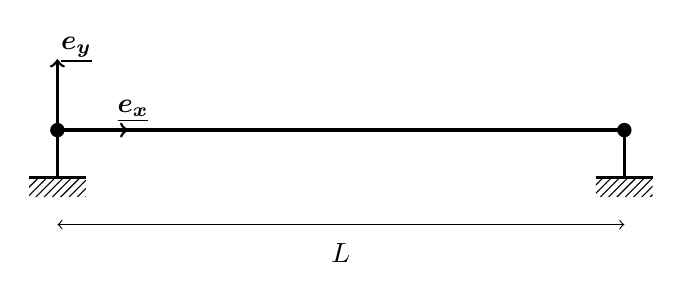
\begin{tikzpicture}[scale=1.2]
  % Beam
  \draw[line width=1.5pt] (0,0) -- (6,0);
  
  % Left support (pin)
  \draw[fill=black] (0,0) circle (2pt);
  \draw[line width=1pt] (0,0) -- (0,-0.5);
  \fill[pattern=north east lines] (-0.3,-0.5) rectangle (0.3,-0.7);
  \draw[line width=1pt] (-0.3,-0.5) -- (0.3,-0.5);
  
  % Right support (roller)
  \draw[fill=black] (6,0) circle (2pt);
  \draw[line width=1pt] (6,0) -- (6,-0.5);
  \fill[pattern=north east lines] (5.7,-0.5) rectangle (6.3,-0.7);
  \draw[line width=1pt] (5.7,-0.5) -- (6.3,-0.5);
  
  % Dimensions
  \draw[<->] (0,-1.0) -- (6,-1.0);
  \node at (3,-1.3) {$L$};
  
  % Load (optional)
  \draw[->,line width=1pt] (0,0) -- (0,0.75);
  \draw[->,line width=1pt] (0,0) -- (0.75,0);
  \node at (0.8,0.2) {$\underline{\boldsymbol{e_x}}$};
  \node at (0.2,0.85) {$\underline{\boldsymbol{e_y}}$};
  
\end{tikzpicture}
\caption{Simply supported beam configuration}
\label{fig:beam_geometry}
\end{figure}
The work carried out on all of this report was done on a simply supported beam

\subsection{Element type}

Euler Beam elements were used for the discretization of the beam structure. These elements are suitable for slender beams where shear deformation is negligible.
Using 4 Gauss Point for the shape functions integration. The residual is following the principle of virtual work.
\begin{equation}
R = \int_{L} \delta \epsilon^T \sigma dL - \int_{L} \delta u^T b dL - \sum_{i=1}^{nLoad} \delta u_i^T Q_i
\end{equation}
\subsection{Material properties}
Unit mass, unit loacal inertia, Young's modulus of 210e9 Pa and a cross section of 0.01 m2 were used for the beam.
Make a table of the properties used.
\begin{table}[htbp]
\caption{Material properties}
\begin{center}
\begin{tabular}{|c|c|c|c|}
\hline
\textbf{Table}&\multicolumn{3}{|c|}{\textbf{Table Column Head}} \\
\cline{2-4} 
\textbf{Head} & \textbf{\textit{Table column subhead}}& \textbf{\textit{Subhead}}& \textbf{\textit{Subhead}} \\
\hline
copy& & &  \\
\hline
\end{tabular}
\label{tab1}
\end{center}
\end{table}
\subsection{Model}

\subsection{Load Scenarii}

\subsection{Inverse simulation}

\section{Results}
\subsection{Inverse crime}


\section{Conclusion}





\begin{thebibliography}{00}
\bibitem{b1} G. Eason, B. Noble, and I. N. Sneddon, ``On certain integrals of Lipschitz-Hankel type involving products of Bessel functions,'' Phil. Trans. Roy. Soc. London, vol. A247, pp. 529--551, April 1955.
\bibitem{b2} J. Clerk Maxwell, A Treatise on Electricity and Magnetism, 3rd ed., vol. 2. Oxford: Clarendon, 1892, pp.68--73.
\bibitem{b3} I. S. Jacobs and C. P. Bean, ``Fine particles, thin films and exchange anisotropy,'' in Magnetism, vol. III, G. T. Rado and H. Suhl, Eds. New York: Academic, 1963, pp. 271--350.
\bibitem{b4} K. Elissa, ``Title of paper if known,'' unpublished.
\bibitem{b5} R. Nicole, ``Title of paper with only first word capitalized,'' J. Name Stand. Abbrev., in press.
\bibitem{b6} Y. Yorozu, M. Hirano, K. Oka, and Y. Tagawa, ``Electron spectroscopy studies on magneto-optical media and plastic substrate interface,'' IEEE Transl. J. Magn. Japan, vol. 2, pp. 740--741, August 1987 [Digests 9th Annual Conf. Magnetics Japan, p. 301, 1982].
\bibitem{b7} M. Young, The Technical Writer's Handbook. Mill Valley, CA: University Science, 1989.
\end{thebibliography}

\end{document}